% CS / code listings and related diagrams (reusable; not exam-specific). Load after \texttt{xcolor}.

\usepackage{graphicx}
\usepackage{ulem}
\usepackage{listings}
\usepackage{array}
\usepackage{tikz}
\usetikzlibrary{arrows.meta}

% --- AP CSP-style pseudocode (\texttt{cs-p/*.tex}) ---
\lstdefinestyle{csppseudo}{%
  basicstyle=\ttfamily\footnotesize,
  keywordstyle=\bfseries\color{blue!55!black},
  commentstyle=\itshape\color{black!50},
  stringstyle=\color{green!50!black},
  columns=fullflexible,
  keepspaces=true,
  tabsize=2,
  showstringspaces=false,
  breaklines=true,
  breakatwhitespace=true,
  frame=single,
  rulecolor=\color{black!35},
  backgroundcolor=\color{black!4},
  frameround=tttt,
  xleftmargin=0.9em,
  xrightmargin=0.5em,
  aboveskip=\smallskipamount,
  belowskip=\smallskipamount,
  numbers=left,
  numberstyle=\scriptsize\color{black!45},
  numbersep=7pt,
  morekeywords={%
    PROCEDURE,REPEAT,UNTIL,TIMES,IF,ELSE,RETURN,DISPLAY,%
    LENGTH,RANDOM,MOVE_FORWARD,ROTATE_LEFT,MOVE_BACKWARD,ROTATE_RIGHT,%
    REMOVE,FOR,TO,WHILE,EACH,IN,APPEND,IsFound,CAN_MOVE,GoalReached,%
    AND,OR,NOT,true,false,min,max,MIN,MAX%
  },
  sensitive=false,
}
\lstnewenvironment{cspcode}{\lstset{style=csppseudo}}{}

% --- Java (CS-A) ---
\lstdefinestyle{javaexam}{%
  language=Java,
  basicstyle=\ttfamily\footnotesize,
  keywordstyle=\bfseries\color{blue!55!black},
  commentstyle=\ttfamily\color{black!50},
  stringstyle=\color{green!50!black},
  columns=fullflexible,
  keepspaces=true,
  tabsize=2,
  showstringspaces=false,
  breaklines=true,
  breakatwhitespace=true,
  frame=single,
  rulecolor=\color{black!35},
  backgroundcolor=\color{black!4},
  xleftmargin=0.5em,
  xrightmargin=0.5em,
  aboveskip=4pt,
  belowskip=4pt,
}

\lstdefinestyle{javainline}{%
  language=Java,
  basicstyle=\ttfamily,
  keywordstyle=\bfseries\color{blue!55!black},
  commentstyle=\ttfamily\color{black!50},
  stringstyle=\color{green!50!black},
  columns=fullflexible,
  keepspaces=true,
  showstringspaces=false,
}

% --- SQL ---
\lstdefinelanguage{SQLEXAM}{%
  morekeywords={%
    SELECT,FROM,WHERE,INSERT,INTO,VALUES,DELETE,UPDATE,ALTER,TABLE,ADD,DROP,%
    CREATE,TRUNCATE,VIEW,GROUP,BY,ORDER,HAVING,AND,OR,NOT,NULL,PRIMARY,KEY,%
    FOREIGN,REFERENCES,JOIN,INNER,LEFT,RIGHT,FULL,OUTER,CROSS,NATURAL,ON,AS,%
    CHECK,UNIQUE,DEFAULT,SERIAL,CASCADE,SET,COMMIT,ROLLBACK,SAVEPOINT,INDEX,%
    MODIFY,COLUMN,DISTINCT,LIMIT,OFFSET,LIKE,IN,BETWEEN,IS,%
  },%
  sensitive=false,%
  morecomment=[l]--,%
  morestring=[b]',%
}%
\lstdefinestyle{sqlinline}{%
  language=SQLEXAM,
  basicstyle=\ttfamily,
  keywordstyle=\bfseries\color{blue!55!black},
  commentstyle=\ttfamily\color{black!50},
  stringstyle=\color{green!50!black},
  columns=fullflexible,
  keepspaces=true,
  showstringspaces=false,
}%
\lstdefinestyle{sqlexam}{%
  language=SQLEXAM,
  basicstyle=\ttfamily\footnotesize,
  keywordstyle=\bfseries\color{blue!55!black},
  commentstyle=\ttfamily\color{black!50},
  stringstyle=\color{green!50!black},
  columns=fullflexible,
  keepspaces=true,
  showstringspaces=false,
  breaklines=true,
  breakatwhitespace=true,
  frame=single,
  rulecolor=\color{black!35},
  backgroundcolor=\color{black!4},
  xleftmargin=0.5em,
  xrightmargin=0.5em,
  aboveskip=4pt,
  belowskip=4pt,
}%

% --- Maven \texttt{pom.xml} ---
\lstdefinestyle{pomxml}{%
  language=XML,
  numbers=none,
  basicstyle=\ttfamily\footnotesize,
  keywordstyle=\bfseries\color{blue!55!black},
  stringstyle=\color{green!50!black},
  columns=fullflexible,
  keepspaces=true,
  tabsize=4,
  showstringspaces=false,
  breaklines=true,
  breakatwhitespace=true,
  frame=single,
  rulecolor=\color{black!35},
  backgroundcolor=\color{black!4},
  xleftmargin=0.5em,
  xrightmargin=0.5em,
  aboveskip=4pt,
  belowskip=4pt,
}%

% --- HTML / CSS / JS ---
\lstdefinelanguage{CSSEXAM}{%
  morekeywords={%
    color,background,background-color,margin,padding,border,border-width,%
    border-style,border-color,width,height,display,font,font-size,font-style,%
    font-weight,text-align,text-decoration,box-sizing,position,overflow,%
    opacity,max-width,min-width,flex,align-items,justify-content,gap,z-index},%
  sensitive=false,%
  morecomment=[s]{/*}{*/},%
  morestring=[b]',%
}%
\lstdefinelanguage{JSEXAM}{%
  morekeywords={%
    break,case,catch,class,const,continue,debugger,default,delete,do,else,%
    export,extends,false,finally,for,function,if,import,in,instanceof,new,%
    null,return,super,switch,this,throw,true,try,typeof,var,void,while,%
    let,static,async,await,of,yield},%
  sensitive=true,%
  morecomment=[l]{//},%
  morecomment=[s]{/*}{*/},%
  morestring=[b]',%
  morestring=[b]"% 
}%
\lstdefinestyle{htmlexam}{%
  language=HTML,
  basicstyle=\ttfamily\footnotesize,
  keywordstyle=\bfseries\color{blue!55!black},
  commentstyle=\ttfamily\color{black!50},
  stringstyle=\color{green!50!black},
  columns=fullflexible,
  keepspaces=true,
  tabsize=2,
  showstringspaces=false,
  breaklines=true,
  breakatwhitespace=true,
  frame=single,
  rulecolor=\color{black!35},
  backgroundcolor=\color{black!4},
  xleftmargin=0.5em,
  xrightmargin=0.5em,
  aboveskip=4pt,
  belowskip=4pt,
}%
\lstdefinestyle{cssexam}{%
  language=CSSEXAM,
  basicstyle=\ttfamily\footnotesize,
  keywordstyle=\bfseries\color{blue!55!black},
  commentstyle=\ttfamily\color{black!50},
  stringstyle=\color{green!50!black},
  columns=fullflexible,
  keepspaces=true,
  tabsize=2,
  showstringspaces=false,
  breaklines=true,
  breakatwhitespace=true,
  frame=single,
  rulecolor=\color{black!35},
  backgroundcolor=\color{black!4},
  xleftmargin=0.5em,
  xrightmargin=0.5em,
  aboveskip=4pt,
  belowskip=4pt,
}%
\lstdefinestyle{jsexam}{%
  language=JSEXAM,
  basicstyle=\ttfamily\footnotesize,
  keywordstyle=\bfseries\color{blue!55!black},
  commentstyle=\ttfamily\color{black!50},
  stringstyle=\color{green!50!black},
  columns=fullflexible,
  keepspaces=true,
  tabsize=2,
  showstringspaces=false,
  breaklines=true,
  breakatwhitespace=true,
  frame=single,
  rulecolor=\color{black!35},
  backgroundcolor=\color{black!4},
  xleftmargin=0.5em,
  xrightmargin=0.5em,
  aboveskip=4pt,
  belowskip=4pt,
}%

% --- Plain HTTP traces ---
\lstdefinestyle{http}{%
  basicstyle=\ttfamily\footnotesize,
  frame=single,
  framerule=0.4pt,
  framesep=3pt,
  xleftmargin=2pt,
  xrightmargin=2pt,
  breaklines=true,
  breakatwhitespace=true,
  columns=fullflexible,
  keepspaces=true,
  aboveskip=4pt,
  belowskip=4pt,
}

\lstset{style=javainline}

% Side-by-side request/response (\texttt{rest.tex}); do not pass \texttt{lstlisting} through a macro argument.
\tikzset{%
  http@arrow/.style={%
    -{Stealth[scale=0.88]}, semithick, shorten >=0.5pt, shorten <=0.5pt, draw=black!55},
}
\newenvironment{httpexchange}{%
  \par\medskip
  \begingroup
  \hfuzz=30pt\relax
  \begin{center}%
  \noindent
  \begin{tabular}{@{} m{0.4\linewidth} >{\centering\arraybackslash}m{1.28cm} m{0.4\linewidth} @{}}%
}{%
  \end{tabular}%
  \end{center}%
  \endgroup
  \medskip
}
\newcommand{\httpmidarrows}{%
  &
  \begin{minipage}[c]{1.28cm}%
    \centering
    \normalfont\footnotesize REQ\par\vspace{1pt}%
    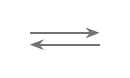
\begin{tikzpicture}[x=1cm, y=0.75cm]
      \draw[http@arrow] (0,0.1) -- (0.92,0.1);
      \draw[http@arrow] (0.92,-0.1) -- (0,-0.1);
    \end{tikzpicture}\par\vspace{1pt}%
    \normalfont\footnotesize RESP%
  \end{minipage}%
  &
}
